\chapter{Desarrollo}

\section{Conocimientos previos y definiciones}
En esta sección se mostrarán las principales nociones de Topología Computacional, que nos darán el contexto y conocimientos necesarios para poder comprender el Teorema de Estabilidad y ser capaces de abordar su demostración.

\subsection{Motivación}
La Topología se centra en en el estudio de las diversas propiedades de los espacios topológicos y las funciones continuas. Mientras que en el subcampo de la Topología Computacional veremos como podemos hacer uso de diversos algoritmos para poder estudiar las propiedades de los espacios topológicos y ser capaces de resolver problemas topológicos computacionalmente. Para ello lo primero que necesitamos es una manera de representación de nuestros espacios topológicos, manteniendo sus propiedades topológicas.

\subsection{Complejos Simpliciales}
Una de las formas de representar un espacio topológico es a través de la descomposición del mismo en piezas más sencillas. Una descomposición en un complejo si sus piezas son topologicamente simples y sus intersecciones son piezas de dimensión inferior del mismo tipo \cite{EH}. Dentro de los complejos se puede observar que hay una gran variedad de tipos, dandonos distintos grados de abstracción. Nosotros vamos a trabajar con los complejos simpliciales, ya que nos darán unas buenas capacidades de computación.

Los complejos simpliciales los podemos estudiar desde un enfoque geométrico y desde un enfoque combinatorio. Partiremos de la definición de complejo simplicial desde el punto de vista geométrico. Para ello recordaremos algunos conceptos de geometría afín.

\begin{definition}
El conjunto de puntos $\{u_0, u_1, ..., u_k\}$ de $\mathbb{R}^d$ es afínmente independiente si los vectores $\{\overrightarrow{u_0u_1}, ..., \overrightarrow{u_0u_k}\}$ son linealmente independientes.
\end{definition}

\begin{definition}
Diremos que $x \in \mathbb{R}^d$ es combinación convexa de los puntos $u_0, u_1, ..., u_k$ si $x = \sum_{i=0}^{k} \lambda_i u_i$ con $\lambda_i \geq 0 \ \forall i \in \{0,...,k\}$ y $\sum_{i=0}^{k} \lambda_i = 1$.
\end{definition}

Llameremos \textbf{envolvente convexa} de $u_0, u_1, ..., u_k$, denotado por $conv\{u_0, u_1, ..., u_k\}$, al conjunto de todas las combinaciones convexas de dichos puntos. Y haciendo uso de este conjunto podremos definir nuestras piezas de la descomposición de la siguiente manera:

\begin{definition}
Un $\bm{k}$\textbf{\textit{-símplice}} $\sigma$ en $\mathbb{R}^d$ con $d \geq k$ es la envolvente convexa de $k+1$ puntos afínmente independientes  $u_0, u_1, ..., u_k \in \mathbb{R}^d$, es decir,
$\sigma \coloneqq conv\{u_0, u_1, ..., u_k\}$
\end{definition}

Diremos que el $k$-símplice $\sigma$ tiene dimensión $k$ y llamaremos \textbf{vértices de} $\bm{\sigma}$ a los puntos $u_0, u_1, ..., u_k$.

\begin{figure}[h]
\centering
\begin{subfigure}[b]{0.2\textwidth}
\centering
   
\begin{tikzpicture}[thick, scale=0.7]
    	\tikzstyle{point}=[circle,thick,draw=black,fill=black,inner sep=0pt,minimum width=4pt,minimum height=4pt]
    	\node (a)[point] at (0,0) {};
    \end{tikzpicture}
    \caption{0-símplice}\label{ref:0simp}
\end{subfigure}
\begin{subfigure}[b]{0.2\textwidth}
\centering
	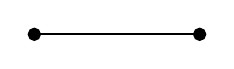
\begin{tikzpicture}[thick, scale=0.7]
    	\tikzstyle{point}=[circle,thick,draw=black,fill=black,inner sep=0pt,minimum width=4pt,minimum height=4pt]
    	\node (a)[point] at (0,0) {};
    	\node (b)[point] at (3,0) {};
 
    	\draw (a.center) -- (b.center) --cycle;
	\end{tikzpicture}
	\caption{1-símplice}\label{ref:1simp}
\end{subfigure}\hspace{0.05\textwidth}
\begin{subfigure}[b]{0.2\textwidth}
\centering
	\begin{tikzpicture}[thick, scale=3]
    	\tikzstyle{point}=[circle,thick,draw=black,fill=black,inner sep=0pt,minimum width=4pt,minimum height=4pt]
    	\node (a)[point] at (0,0) {};
    	\node (b)[point] at (1,0) {};
    	\node (c)[point] at (0.6,0.5) {};

    	\draw[fill=greeo,opacity=0.6] (a.center) -- (b.center) -- (c.center) -- cycle;
 
    	\draw (a.center) -- (b.center) -- (c.center)  --cycle;
	\end{tikzpicture}
	\caption{2-símplice}\label{ref:2simp}
\end{subfigure}\hspace{0.05\textwidth}
\begin{subfigure}[b]{0.2\textwidth}
\centering
	\begin{tikzpicture}[thick,scale=3]
    	\tikzstyle{point}=[circle,thick,draw=black,fill=black,inner sep=0pt,minimum width=4pt,minimum height=4pt]

	\node (A1)[point] at (0,0) {};
	\node (A3)[point] at (1,0) {};
	\node (A4)[point] at (0.4,-0.3) {};
	\node (B1)[point] at (0.5,0.5) {};

	\draw[thick,dashed,opacity=0.6] (A1) -- (A3);
	\draw[fill=greeo,opacity=0.6] (A1.center) -- (A4.center) -- (B1.center) -- cycle;
	\draw[fill=greeo,opacity=0.6] (A3.center) -- (A4.center) -- (B1.center) -- cycle;

	\draw (A1) -- (B1)  -- (A3) -- (A4) --(A1) --cycle;
	\end{tikzpicture}
	\caption{3-símplice}\label{ref:3simp}
\end{subfigure}
\caption{Representación de los símplices de dimensión 0, 1, 2 y 3}
\end{figure}

Se puede observar que cualquier subconjunto de los vértices de $\sigma$ será afínmente independiente y por lo tanto definirá un símplice $\tau$. De esta forma diremos que $\bm{\tau}$ \textbf{es una cara de} $\bm{\sigma}$ si es una convinación convexa de un subconjunto no vacío de los vértices de $\sigma$, y lo denotaremos por $\tau \leq \sigma$. Si el subconjunto es propio, diremos que $\bm{\tau}$ \textbf{es cara propia de} $\bm{\sigma}$, y lo denotaremos por $\tau < \sigma$. Por otro lado, diremos que $\bm{\sigma}$ \textbf{es cocara (propia) de} $\bm{\tau}$ si $\sigma \geq \tau$ ($\sigma > \tau$).

Una vez que ya conocemos las piezas de nuestra descomposicón vamos a ver como tenemos que unirlas y cuales son las principales propiedades de los complejos resultantes.\\
Como ya hemos visto al principio de la sección, para que una descomposición sea un complejo sus piezas tienen que ser topológicamente simples y sus intersecciones tienen que ser piezas de dimensión inferior del mismo tipo. Es por esto que la manera que tendremos que unir unos símplices con otros por sus caras.

\begin{definition}
Un \textbf{complejo simplicial} es una colección finita de símplices $K$ que satisface las siguientes propiedades:
\begin{enumerate}
	\item Si $\sigma \in K$ y $\tau \leq \sigma$ entonces $\tau \in K$.
	\item Si $\sigma_0,\sigma_1 \in K$ y $\sigma_0 \cap \sigma_1 \neq \emptyset$ entonces $\sigma_0 \cap \sigma_1 \leq \sigma_i$ para $i = 1,2$.
\end{enumerate}
\end{definition}

Se define la dimensión de como el máximo de las dimensiones de sus símplices.

Un ejemplo de complejo simplicial es lo que se muestra en la figura \ref{ref:comp1}, mientras que en la figura \ref{ref:noComp} muestra un ejemplo que no es complejo simplicial.


\begin{figure}[ht]
\centering
\begin{tikzpicture}[thick,scale=3]
    	\tikzstyle{point}=[circle,thick,draw=black,fill=black,inner sep=0pt,minimum width=4pt,minimum height=4pt]


	\node (x)[point] at (0,0) {};

	\node (A1)[point] at (1,0) {};
	\node (A3)[point] at (2, 0.1) {};
	\node (A4)[point] at (1.4,-0.3) {};
	\node (B1)[point] at (1.5,0.5) {};

    \node (b)[point] at (3,0) {};
    \node (c)[point] at (2.6,-0.5) {};
    
    \node (a1)[point] at (3.4,0.12) {};
    \node (b1)[point] at (4,0) {};
    \node (c1)[point] at (3.8,0.3) {};
    
    \node (y)[point] at (3.5,-0.4) {};

    \draw[fill=greeo,opacity=0.6] (a1.center) -- (b1.center) -- (c1.center) -- cycle;
    \draw (a1.center) -- (b1.center) -- (c1.center)  --cycle;

	\draw[thick,dashed,opacity=0.6] (A1) -- (A3);

	\draw[fill=greeo,opacity=0.6] (A1.center) -- (A4.center) -- (B1.center) -- cycle;
	\draw[fill=greeo,opacity=0.6] (A3.center) -- (A4.center) -- (B1.center) -- cycle;

	\draw (A1) -- (B1)  -- (A3) -- (A4) --(A1) --cycle;
	
	\draw (x.center) -- (A1.center) --cycle;	
	\draw (A3.center) -- (b.center) -- (c.center)  --cycle;	
	
	\draw (b1.center) -- (y.center) --cycle;
		
	\end{tikzpicture}
\caption{Ejemplo de complejo simplicial}
\label{ref:comp1}
\end{figure}

\begin{figure}[ht]
\centering
\begin{tikzpicture}[thick]
    \tikzstyle{point}=[circle,thick,draw=black,fill=black,inner sep=0pt,minimum width=4pt,minimum height=4pt]
    \node (a)[point] at (0,0) {};
    \node (b)[point] at (3,0) {};
    \node (c)[point] at (2,2) {};

    \begin{scope}[yshift=2cm]
    \node (d)[point] at (1,1) {};
    \node (e)[point] at (0,2) {};
    \node (f)[point] at (4,2) {};
    \end{scope}

    \draw[fill=greeo,opacity=0.6] (a.center) -- (b.center) -- (c.center) -- cycle;
    \draw[fill=greeo,opacity=0.6] (d.center) -- (e.center) -- (f.center) -- cycle;
    \node (p)[point] at (1.5,0.5) {};
 
    \draw (p.center) -- (d.center);
    \draw (a.center) -- (b.center) -- (c.center)  --cycle;
    \draw (d.center) -- (e.center) -- (f.center) -- cycle;
\end{tikzpicture}
\caption{Ejemplo de conjunto de símplices que no cumplen las condiciones de complejo simplicial}
\label{ref:noComp}
\end{figure}

El \textbf{espacio subyacente} de un complejo simplicial $K$, denotado $\abs{K}$, es la unión de los símplices de $K$ con la topología heredada del $\mathbb{R}^d$ donde viven sus símplices. Este espacio subyacente también es llamado \textbf{poliedro}. Como se puede observar, el espacio subyacente  de un complejo simplicial es compacto, el cual es un resultado que nos será necesario para la demostración del Teorema de Estabilidad.

Una vez que conocemos como se definen los complejos simpliciales y su correspondiente topología, vamos a ver como vincular un espacio topológico con un complejo simplicial. Para ello haremos uso de las triangulaciones:

\begin{definition}
Una \textbf{triangulación} de un espacio topológico $X$ es un par $(K, h)$ donde $K$ es un complejo simplicial y $h: X \longrightarrow \abs{K}$ es un homeomorfismo ($h$ continua, biyectiva y $h^{-1}$ continua).
\end{definition}
Diremos que un espacio topológico es \textbf{triangulable} si admite una triangulación. Y por tanto, los espacios $\abs{K}$ y $X$ son iguales (topologicamente hablando).

También nos será de utilidad poder estudiar los complejos simpliciales contenidos en otro complejo simplicial.
\begin{definition}
Un \textbf{subcomplejo} $L$ de un complejo simplicial $K$ es un complejo simplicial $L \subseteq K$.
\end{definition}

Un subcomplejo de gran interés son los $\bm{j}$\textbf{-esqueletos}, definidos de la siguiente forma: \[K^{(j)} = \{\sigma \in K : dim\ \sigma\ \leq j\}\]

Otro subconjunto de símplices que nos será de gran ayuda más adelante es la \textbf{estrella de un símplice} $\bm{\tau}$, la cual consiste de las cocaras de $\tau$, denotado por $St(\tau)$. Este conjunto no será siempre un complejo simplicial, así que se define la \textbf{estrella cerrada} $\overline{St}(\tau)$ como el menor subcomplejo de $K$ que contiene a $St(\tau)$. Adicionalmente, se define el \textbf{link} de $\tau$ como: $Lk(\tau) = \{\tau \in \overline{St}(\tau): \sigma \cap \tau = \emptyset\}$.

\subsubsection*{complejo simplicial abstracto: esquema de vertices, realización geométrica y teorema}
\subsubsection*{def subdivisión de un complejo simplicial}
\subsubsection*{subdivisión baricéntrica: def y lema}
\subsubsection*{aplicaciones simpliciales y aproximaciones simpliciales}

Desde el punto de vista computacional nos encontramos con el problema de que tenemos una representación de un espacio topológico a través de una discretización finita de los puntos de dicho espacio, y nuestro objetivo es poder recuperar las propiedades del espacio topológico original a partir de esta nube de puntos. Para ello usaremos complejos simpliciales asociados a dicha nube de puntos.

\subsubsection*{def complejo de \v{C}ech}
\subsubsection*{def complejo de Vietoris-Rips}
\subsubsection*{def diagrama de Voronoi + triangulación Delonay}
\subsubsection*{def alpha complejo}

\subsection{Homología}
Como se puede ver en [añadir cita] la homotopía es una gran herramienta algebraica para poder obtener propiedades de los espacios topológicos. Sin embargo, los métodos para el cálculo de la homotopía no son los mejores computacionalmente. Así pues, se propone la homología como formalismo algebraico, que aunque no es capaz de obtener tanta información topológica sobre el espacio como con otros formalismos, contiene algoritmos mucho más rápidos y eficientes.


\subsubsection*{grupos de cadenas}
\subsubsection*{operador borde: complejos de cadenas, ciclos y bordes}
\subsubsection*{grupos de homología simplicial: definición, números de betti, caracteristica de euler, teorema de conexion y numeros de betti}
\subsubsection*{aplicaciones inducidas para grupos de homología}

\subsubsection*{Homología singular}
Comentar existencia de la homología singular y el porqué se creó y que beneficios, pero debido a que el teorema de estabilidad parte de un espacio topológico triangulable no es necesario


\textit{HERBERT EDELSBRUNNER AND JOHN HARER: PERSISTENT HOMOLOGY — A SURVEY\\}
``REMARK 2.1. There are a variety of other homology theories defined in topology.
Most notably singular homology has the advantage that it exists for arbitrary topological
spaces and it is easy to define concepts like induced maps, prove that homotopy equivalent
maps induce isomorphisms on homology, etc. However, in singular homology the chain
groups are infinite-dimensional and therefore not directly suited to computational methods.
Nevertheless, the reader should be aware of this theory. It justifies the common practice of
talking about homology for spaces without an explicit triangulation. Most of the time, and
certainly in low dimensions, singular and simplicial homology are equivalent theories.''

\textit{Crossley, Martin D., Essential Topology. Springer-Verlag, London, 2005.\\}
``For simplicial homology we supposed that our space had already been expressed as a simplicial complex, i.e., decomposed into a union of simplices. Some spaces cannot be expressed in such a way, and even those that can, can usually be expressed as a simplicial complex in many different ways. Choosing one way can obscure some details of the space. For these reasons “singular” homology was developed, which gets around this problem by, in a very loose sense, considering all possible simplicial decompositions.''

\subsection{Persistencia}

\subsubsection*{funciones reales}
poder ver graficamente como a traves de las contraimagenes se generan diferentes componentes al pasar por puntos criticos
\subsubsection*{funciones morse} 
def variedad diferenciable, definición de las funciones morse, ver como la homología cambia al pasar por los puntos críticos y ver las nociones de nacimiento y muerte
\subsubsection*{funciones tame}
definicion función tame, subniveles, grupos de persistencia a partir de funciones tame, critical value lema,  numeros de betti de grupos de persistencia y su relación con las multiplicidades.

Definición de diagrama de persistencia, k-triangle lemma


\subsubsection*{persistencia en complejos simpliciales}
particularizar lo visto en funciones tame pero con complejos simpliciales

\subsubsection*{funciones PL}
definición de las funciones pl, generación de filtraciones a partir del lower star filtration y estudio de los puntos criticos  de las funciones pl para comprobar que son funciones tame.



